\documentclass{book}
    \usepackage[italian]{babel}
    \usepackage[utf8]{inputenc}
    \usepackage[T1]{fontenc}
%%%%% Pacchetti
\usepackage{FileAusiliari/Layout}			% Contiene i pacchetti e le impostazioni per il layout
\usepackage{FileAusiliari/Pacchetti}		% Pacchetti aggiuntivi di vario tipo (senza tikz)
\usepackage{FileAusiliari/TikZ}				% Ambiente tikzpicture
\usepackage{FileAusiliari/Definizioni}		% Definizioni di colori, variabili globali ecc.
\usepackage{FileAusiliari/Environments}		% Impostazioni TOC, bibliografia e indice analitico + environments vari per il contenuto del documento
\usepackage{FileAusiliari/Custom}			% Tutto ciò che è personalizzabile normalmente dall'utente (tranne i colori per collegamenti ipertestuali, citazioni, link, che sono da modificare in Referencing)
\usepackage{FileAusiliari/Referencing}		% Collegamenti ipertestuali e indice analitico
\usepackage{FileAusiliari/Comandi}			% Comandi vari
%%%%%%%%%%%%%%%%%%%%%%%%%%%%
%%%%%%%%%%%%%%%%%%%%%%%%%%%%
\begin{document}
%%%%%%%%%%%%%%%%%%%%%%%%%%%%									 TITOLO
%%%%%%%%%%%%%%%%%%%%%%%%%%%%
\begin{titlepage}
	
    \raggedleft	

    \rule{1pt}{.9\textheight}
	\hspace{0.075\textwidth}
	\parbox[b]{.85\textwidth}{
		{\HUGE\bfseries Natural Language Processing
        }\\[2\baselineskip]
		{\Large\textit{appunti e note raccolte 2022/2023}}\\[47.5\baselineskip]
        {\Large\textsc{* per ora * fusione appunti di: Paolo Ciasco, Andrea Cantarini, Giulio Appetito, Anastasia Brinati}}\\[1\baselineskip]
        
	}
\end{titlepage}
%%%%%%%%%%%%%%%%%%%%%%%%%%%%									FRONTMATTER
%%%%%%%%%%%%%%%%%%%%%%%%%%%%
\frontmatter
%%%%%								 INDICE
\begingroup
{
	\let\cleardoublepage\relax
	%%%%%		Nome Indice (NASCOSTO E CREATO A PARTE)
	\renewcommand\contentsname{}
	\begin{tikzpicture}[remember picture, overlay]
		\clip (-80,-95) rectangle (40,10);
		\pgftext[x=.8\textwidth, y=0.2cm]{\HUGE\bfseries 
		Indice}						% Titolo indice
		\end{tikzpicture}
	\vspace{-1cm}
	
	\tableofcontents*
	\vspace{.25cm}
}
%%%%%								INTRODUZIONE
		\titleformat{\chapter}
		[hang]
		{\Huge}
		{}
		{0em}
		{}
		[\Large {\begin{tikzpicture} [remember picture, overlay]
		\pgftext[right,x=14.75cm,y=0.2cm]{\HUGE\bfseries 
			Introduzione}
		\end{tikzpicture}}]
%%%%%%%%%%%%%%%%%%%%%%%%%%%%%%%%%%%%%%%%%%%%%%%%%%%%%%%%%%%%%%%%%%%%%%%%%%%%%%%%%
\chapter*{}\normalfont\addcontentsline{toc}{part}{Introduzione}


Lo scopo di questo documento è raccogliere appunti e note degli studenti del corso NLP, e creare un riassunto sostanzioso e fruibile a chiunque negli anni a venire, con la speranza che venga ampliato e modificato da futuri studenti.

"What is natural language and what do we want to do with it?", è la domanda di apertura del corso. Lo scopo del linguaggio è far comunicare due (o più) entità. Secondo Ferdinand De Saussure i parlanti si accordano per chiamare oggetti e concetti in determinate maniere. La ragion d'esistere delle parole non c'è, l'accezione è relativa ad un aspetto sociale. Parliamo infatti di linguistica *esterna*, ovvero studio del linguaggio come entità esterna all’individuo. Distinguiamo inoltre la *langue*, l'entità sociale propria di una comunità, canonizzata e dunque indrottinata ai cervelli, dalla *parole*, che è invece l'entità naturale, espressione con la propria cognizione (=attuazione individuale) della langue.
Chomsky tratta invece della linguistica interna, studio del linguaggio come capacità cognitiva dell’individuo, dove la distinzione è fra *competence*, capacità d apprendere, e *performance*, capacità di produzione del linguaggio.
I large language models lavorano sulla parole, anche se inizialmente l'NLP, le discipline Corpus Linguistics e gli EMNLP (empirical metaods for NLP), si concentravano sulla competence. Anche se la parole evolve continuamente, la langue stessa non è stabile: le parole nascono, muoiono e cambiano di significato. 
\endgroup

%%%%%								ERRATA 
\iffalse
		\titleformat{\chapter}
		[hang]
		{\huge}
		{}
		{0em}
		{}
		[\large {\begin{tikzpicture} [remember picture, overlay]
		\pgftext[right,x=14.75cm,y=0.2cm]{\color{black}\Huge\bfseries 
			Errata corrige \& Aggiunte};
		\end{tikzpicture}}]
\chapter*{}\normalfont		\addcontentsline{toc}{part}{Errata corrige \& Aggiunte}
\begin{longtable}{p{2.55cm}p{1.45cm}p{9cm}}
	Data di \newline correzione & Pagina&\\\hline
	24/10/2023	& ?	& ?
\end{longtable}
\fi

%%%%%%%%%%%%%%%%%%%%%%%%%%%%									MAINMATTER
%%%%%%%%%%%%%%%%%%%%%%%%%%%%
\mainmatter

\titleformat{\chapter}[display]{\bfseries\Large}	{\filleft\MakeUppercase{\chaptertitlename} \HUGE\thechapter}{.5ex}{\titlerule\vspace{.1ex}\filleft}[\vspace{.5ex}]
\titlespacing*{\chapter}{0pt}{0.1\baselineskip}{0.5\baselineskip}

\fancyheadoffset[L]{\dimexpr\oddsidemargin-0in\relax}
\fancyheadoffset[R]{\dimexpr\oddsidemargin-0in\relax}

\normalfont
\normalsize


\newgeometry{top=35mm, bottom=35mm, left=15mm, right=15mm, headheight=0pt, headsep=0pt, marginparsep=0pt, marginparwidth=0pt, footskip=0pt, footnotesep=0pt}
\part*{\HUGE Parte 1}\label{Parte1}
\restoregeometry

%%%%%								CAPITOLI
\chapter{Introduzione al fenomeno della lingua}
\section{Significato e significante}

\begin{abstract}
Il linguaggio è uno strumento per trasmettere informazioni attraverso una serie di simboli. Ma cosa è un simbolo? Dato un oggetto (significato), un simbolo è ciò che lo rappresenta (significante).
I veicoli segnici rappresentano i sensi delle parole (che sono nell'iperuranio/nella testa dei parlanti).
\end{abstract}

\begin{figure}
    \centering
    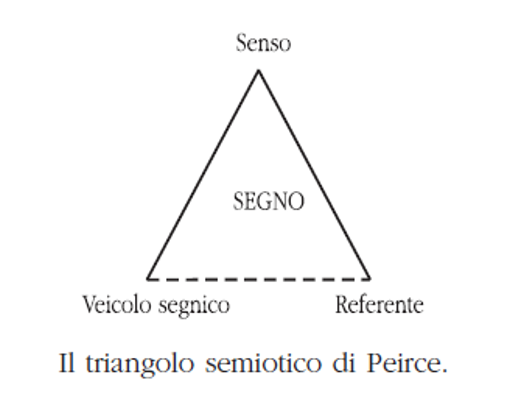
\includegraphics[width=0.5\linewidth]{peirce.PNG}
    \caption{Triangolo di Peirce}
    \label{fig:enter-label}
\end{figure}

\begin{abstract}
Tuttavi andare dal veicolo segnico al senso e viceversa non è immediato poichè la relazione è 'molti a molti', infatti, la rappresentazione naturale soffre di molti "difetti", come ad esempio la ricchezza espressiva(più veicoli segnici vanno in un unico senso), l'arbitrarietà e l'ambiguità (più sensi vanno in uno stesso veicolo segnico).
\begin{Oss}{Esempio:} Una vecchia legge la regola \end{Oss}
Esistono però vari tipi di ambiguità in base al livello linguistico in cui ci troviamo.
\end{abstract}

%%%%%%%%%%%%%%%%%%%%%%%%%%%%%%%%%%%
\section{Livelli linguistici}

\begin{abstract}
Fonologia: branca della linguistica che studia i sistemi di suoni; la più semplice particella che studia la fonologia è il \textbf{fonema}, che può essere un singolo suono.
\end{abstract}

\begin{abstract}
Morfologia: è lo studio delle parole, la loro composizione, e l'appartenenza a determinate categorie (nome, verbo, etc...).
Nella linguistica moderna studia la struttura della parola e descrive le varie forme che assume a seconda delle categorie di numero, genere, modo, tempo e persona.
Le parole sono costituite di \textbf{morfemi}, unità minime con significato autonomo, ..
\end{abstract}

\begin{abstract}
Sinstassi: branca della grammatica e linguistica che studia i diversi modi (relazioni) in cui i codici dei linguaggi si uniscono fra loro per formare una preposizione, "unità superiori alla parola". 
\end{abstract}

\begin{abstract}
Sematica: studio del significato delle parole (lessicale), e delle frasi (frasale), considerando il rapporto fra l'espressione e la realtà extralinguistica. Il significato di una frase è dato da quello delle singole parti, più quello degli eventuali elementi connettori (anche se non è detto che ciò sia sufficiente, considerando ad esempio metafore o catacresi).
\end{abstract}

\begin{abstract}
Pragmatica: studio del linguaggio in rapporto all'uso contestuale che ne fa il parlante, come il contesto contribuisce al significato.
\end{abstract}

%%%%%%%%%%%%%%%%%%%%%%%%%%%%%%%%%%%
\section{Interpreting Natural Language}

\begin{abstract}
Abbiamo stabilito che lo scopo de linguggio naturale è la comunicazione, trasmettere idee sul mondo interiore o esteriore, credenze, knowledge, concetti, emozioni... ma come lo interpretiamo?
Dati dei concetti e le relazioni fra essi vogliamo ricavare istanze, fatti accaduti. -> Retriving information from text collection
Vogliamo definire un meccanismo (finito) che possa generare ed interpretare un linguaggio:
    \begin{itemize}
        \item interpretare: da una frase costruire il grafo(albero) di derivazione;
        \item generare: dal grafo ricostruire la frase;
    \end{itemize}
\end{abstract}

\section{Classi sintattiche e costituenti}
\begin{abstract}
I morfemi si suddividono in chiusi (grammaticali), che permettono di cambiare il gruppo sintattico, e aperti (lessicali), che portano il significato.
\begin{Oss}{Esempio:} (closed, prefix) re - (open) play - (closed, suffix) ing/ed/er \end{Oss}
    qua va messa tutta la roba de introduzione ai costituenti e le classi grammaticali (nomi, verbi, avverbi, etc..)
    cosa è un costituente? come si individua?
    test ai costituenti: scissione, isolabilità e interrompibilità.
    
\end{abstract}

\begin{abstract}
Gli elementi frasali sono derivati dalle categorie grammaticali, per ciascuna creiamo elementi ricorsivamente ricostruibili e non interropibili: i \textbf{sintagmi}, o \textbf{phrases}.
    \begin{itemize}
        \item NP, noun phrase: sintagmi retti da nomi ( AGG+NOUN || ART+AGG+NOUN || NOUN+AGG || ART+NOUN+AGG )
        \item PP, prepositional phrase: sintagmi preposizionali ( PREP+NP )
        \item VP, verbal phrase: sintagmi verbali
        \item A PP, adjective phrase: sintagmi aggettivali
        \item S, sentence: (?)
    \end{itemize}

Seguendo l'idea di Chomsky per cui la sintassi guida l'interpretazione semantica, il nostro scopo è costruire un modello in grado di produrre \textit{suitable syntactic structures} delle frasi in input.

NON SO SE è IL CASO DI METTERE QUI TUTTA LA RPBA DEI COSTITUENTI O MEGLI ODOPO BOH VEDIAMO
\end{abstract}
\chapter{Machine learning}


Qui verranno inserite tutte le brevi digressioni e cenni sul machine learning...



\section{NN: Neural Networks}

\begin{abstract}
Le NN sono modelli per il machine learning costruiti usando principi dell'organizzazione neuronale: un gruppo di nodi interconnesso(neuroni) che si trasmettono segnali.
Una rete neurale impara processando esempi contenenti un input ed un risultato noto/atteso per quell'input, costruendo associazioni probabilistiche e pesate, conservate nella struttura dati stessa  della rete.
Un neurone (artificiale) è una funziona matematica che riceve un input ne esegue una "somma" (con bias) e restituisce un output (es: sigmoid, step func, ...).
\end{abstract}
\begin{figure}
    \centering
    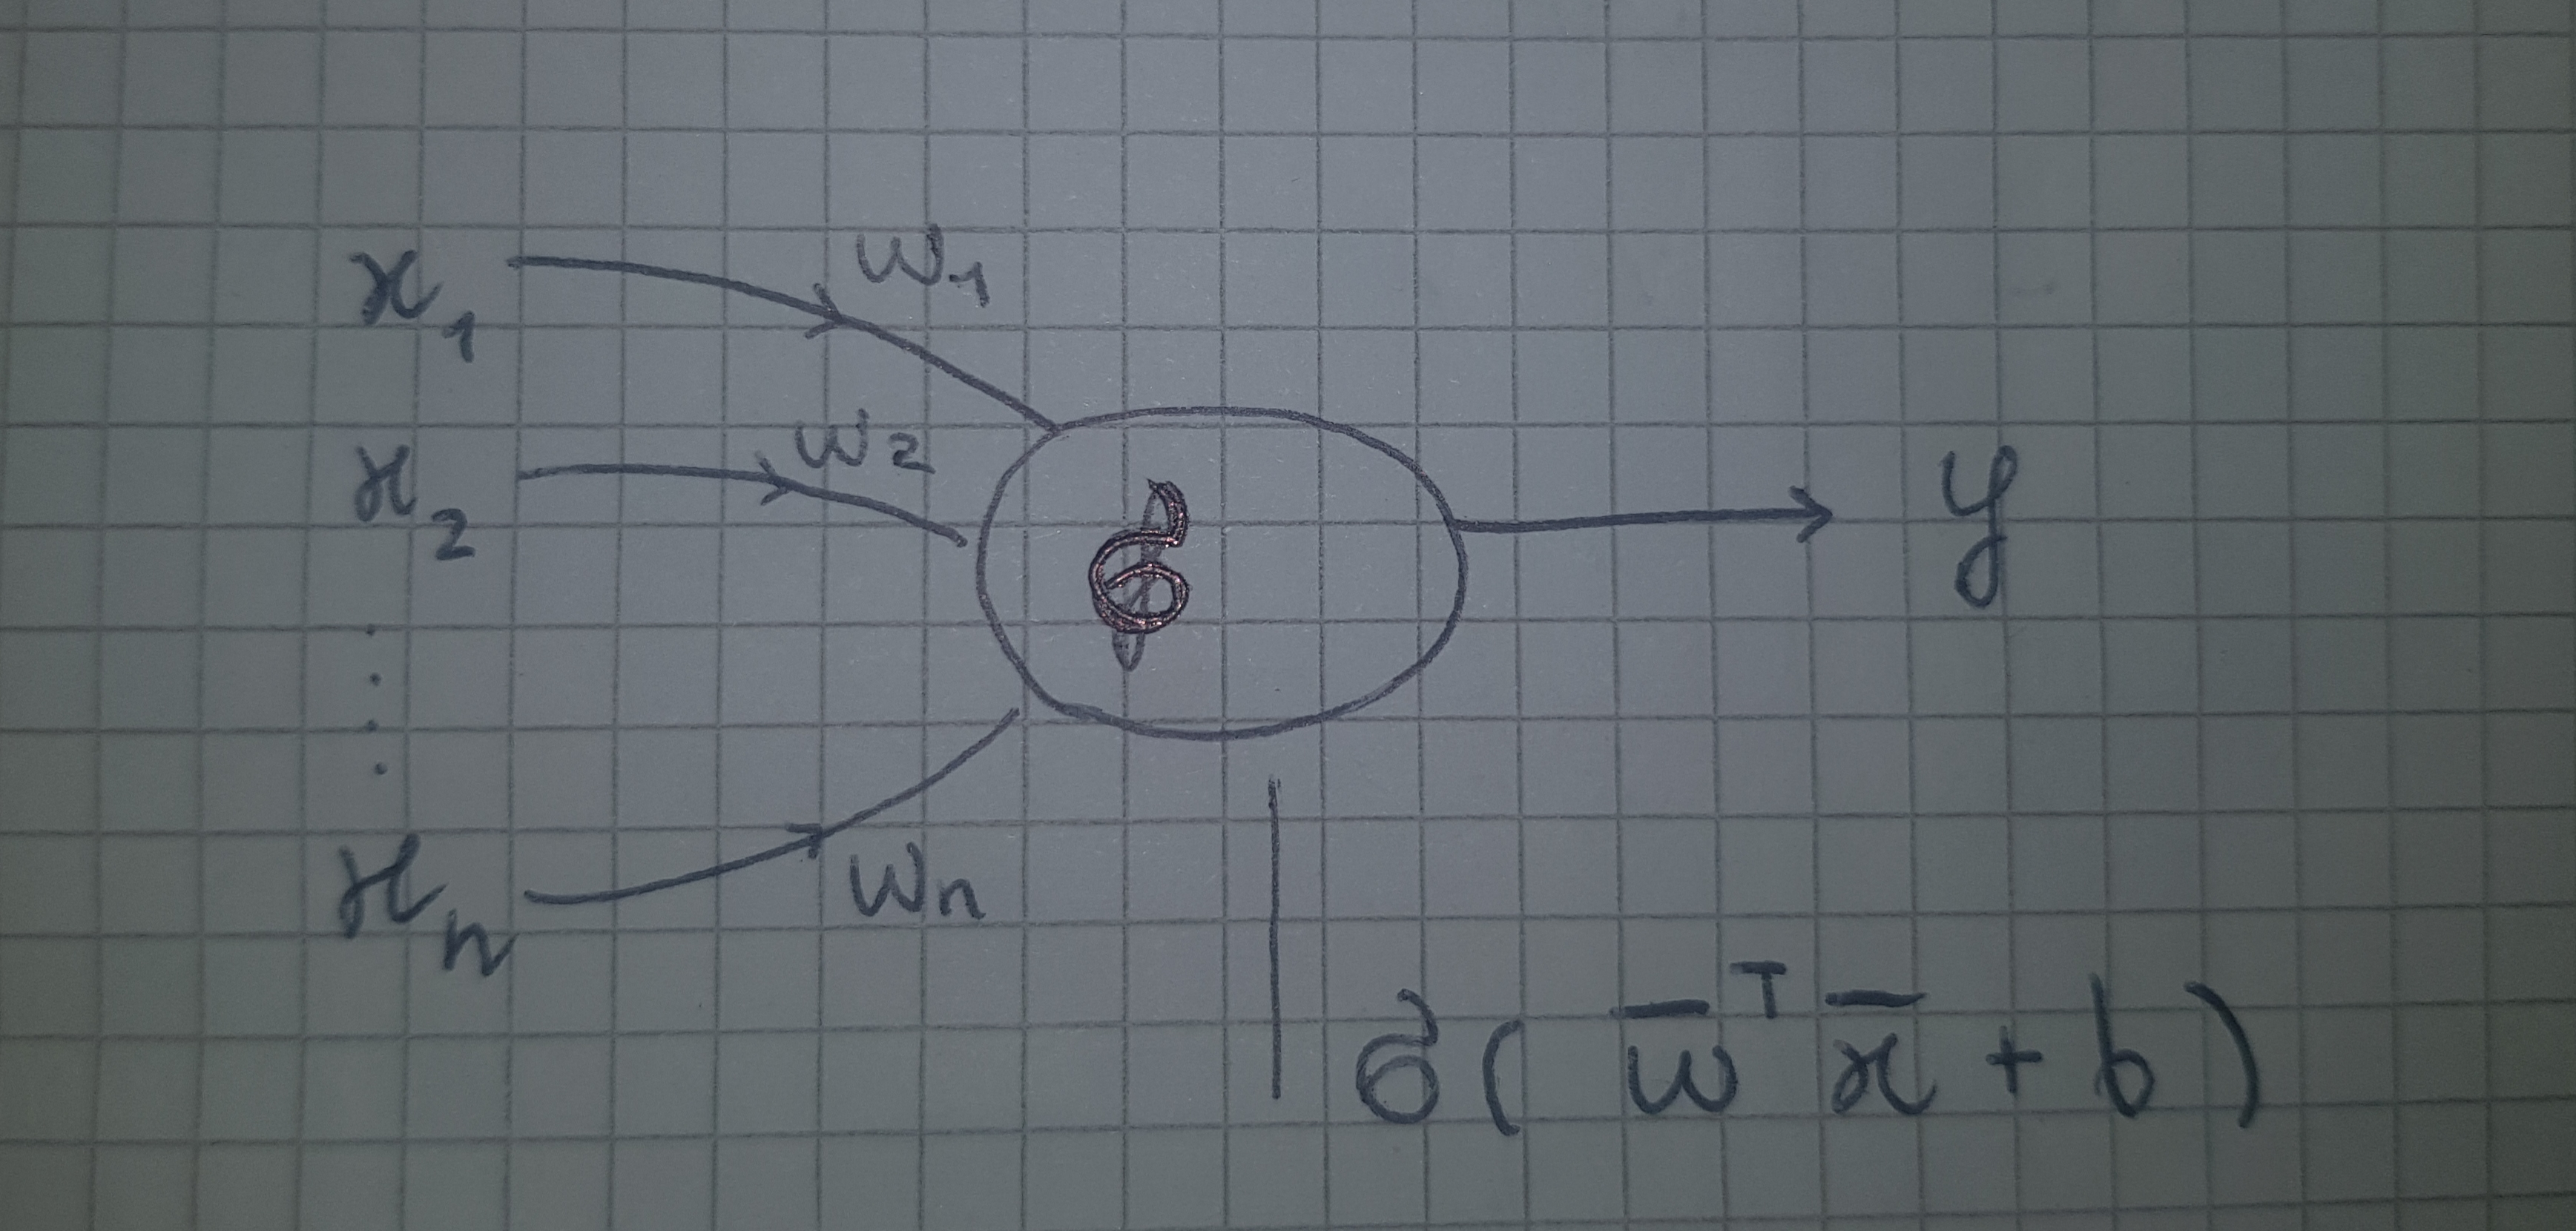
\includegraphics[width=0.5\linewidth]{20231130_172209.jpg}
    \caption{Enter Caption}
    \label{fig:enter-label}
\end{figure}
\usepackage{amsmath}

\chapter{Rappresentazioni dei simboli in vettori}

\section{Introduzione}
Il linguaggio naturale è una rappresentazione simbolica della conoscenza umana, e la composizione di simboli in parole e delle parole in frasi segue le regole che l'ascoltatore e il parlante conoscono. Ad oggi, con l'avanzamento del ML, i simboli discreti stanno scomparendo per essere sostituiti da vettori e tensori: si hanno dunque le cosiddette \textbf{rappresentationi distribuite o distribuzionali}, in cui parole e frasi sono rappresentate come vettori o tensori di numeri reali, e i simboli discreti sopravvivono solo come input e output degli algoritmi. \\
Tuttavia vi è un legame tra le rappresentazioni distribuite e i simboli, in quanto la prima è una approssimazione dei secondi. 

\section{Rappresentazioni Distribuite e Simboliche: Interpretabilità e Composizionalità Concatenativa}
Le \textbf{rappresentazioni distribuite} portano le espressioni simboliche in spazi metrici dove la similarità tra esempi è usata per apprendere regolarità usando algoritmi di machine learning. Date due espressioni simboliche dunque, la loro rappresentazione distribuita dovrebbe cogliere la loro similarità e alcune loro feature. \\\\\textbf{Esempio.} Consideriamo due frasi, \textit{s1="un topo mangia il formaggio"} ed \textit{s2="Un gatto mangia il topo"}, ci sono varie similarità, come numero di parole in comune e realizzazione del patter ANIMALE MANGIA CIBO. Il punto chiave è scegliere o far scegliere a un algoritmo quale sia la migliore rappresentazione per un task specifico.\\\\
Nonostante le rappresentazioni distribuite stiano rimpiazzando le rappresentazioni simboliche discrete, queste sono meno interpretabili dagli umani, dunque dovremmo considerare alcune delle proprietà delle rappresentazioni simboliche potrebbero tornare utili.\\
Innanzitutto le rappresentazioni simboliche discrete sono interpretabili dagli umani perchè i simboli non sono alterati nelle espressioni: un insieme infinito di espressioni può essere ottenuto concatenando un \textbf{insieme finito di simboli di base} in accordo a delle regole di concatenazione, processo durante il quale i simboli non vengono alterati. Usando il principio della \textbf{composizionalità semantica}, il significato delle espressioni può essere ottenuto combinando il significato delle varie parti, e ricorsivamente combinando il significato dell'insieme finito di simboli di base. 
\\\\
\textbf{Esempio.} Sia un insieme di simboli di base \textit{D={mouse,cat,a,swallows,(,)}}, allora plausibili espressioni potrebbero essere del tipo:
\begin{itemize}
    \item $s_1$="a cat swallows a mouse"
    \item $t_1$=((a cat)(swallows(a mouse)))
\end{itemize}dove la seconda è una rappresentazione strutturata ad albero in forma parentetica.\\\\

Le rappresentazioni distribuite però sembrano alterare i simboli quando vengono applicate a input simbolici, e dunque sono meno interpretabili, dal momento che i simboli vengono convertiti in vettori o tensori, che a loro volta vengono trasformati con moltiplicazioni tra matrici o con funzioni non lineari. Sorge dunque il dubbio di quale sia la relazione tra i simboli iniziali e le espressioni delle loro rappresentazioni distribuite, e come queste espressioni vengano modificate durante le operazioni tra matrici o con funzioni nonlineari. \\
La domanda che ci poniamo è dunque se le rappresentazioni distribuite e quelle simboliche siano diverse per via dell'alterazione dei simboli. Per contribuire alla risposta, \textit{Gelder(1990)} ha formalizzato questa proprietà di alterare i simboli con due nozioni di composizionalità: \textbf{composizionalità concatenativa} e \textbf{composizionalità funzionale}.

\subsection{Composizionalità concatenativa}
La composizionalità \textit{concatenativa} spiega in che modo le rappresentazioni dei simboli discreti compongano simboli per ottenere espressioni. Infatti, il modo di combinare simboli è quello di estendere il concetto di \textit{giustapposizione} che fornisce un metodo per connettere simboli consecutivi senza alterarli e formare espressioni. Usando l'\textbf{operatore di concatenazione}, le due frasi sopra diventano: $a \cdot cat \cdot swallows \cdot a \cdot cat$, e $\cdot(\cdot(a,cat),\cdot(swallows,\cdot(a,mouse)))$ che rappresenta un albero. 

\subsection{Composizionalità funzionale}
La composizionalità funzionale spiega la composizionalità nelle rappresentazioni distribuite e nella semantica. Nella composizionalità funzionale, il modo di combinazione è una \textbf{funzione $\Phi$} che dà un processo generale per produrre espressioni dati i suoi costituenti. \\
Le \textbf{local distributed representations} e le \textbf{one-hot encodings} sono il miglior modo per vedere come la \textit{composizionalità funzionale} agisce sulle \textit{rappresentazioni distribuite}. Ricordiamo che dato un insieme di simboli $D$, una rappresentazione distribuita locale mappa l'i-imo simbolo nell'i-imo vettore canonico di $R^N$, dove N è la cardinalità di D.Nella composizionalità funzionale, espressioni del tipo $s=w_1w_w...w_k$ sono ottenute con una funzione $\Phi$ applicata ai vettori $e_{w_1}...e_{w_{k}}$, e questa funzione potrebbe anche essere la semplice somma, che ci dà come risultato un vettore \textbf{bag-of-word}, ma ci sono anche funzioni più complesse, come la \textit{convoluzione circolare}; così però si perde la sequenza dei simboli. Oppure, il \textit{prodotto scalare} tra due espressioni $s_1, s_2$ restituisce il numero di parole in comune. In generale, la funzione $\Phi$ è cruciale per determinare se i simboli saranno riconosciuti e la sequenza preservata. 
\\ \\ 
Le \textit{rappresentazioni distribuite} sono più ambiziose delle \textit{rappresentazioni distribuite locali} perchè cercano si codificare simboli base di $D$ in vettori di $R^d$ dove d è molto minore di n, anche se così si alterano i simboli, data la assenza di link tra simboli e rappresentazioni. In generale, data la rappresentazione locale $\textbf{e}_w$ di un simbolo $w$, l'encoder di una \textit{rappresentazione distribuita} è una matrice $\textbf{W}_{dxn}$ che trasforma $e_w$ in $y_w=W_{dxn}e_w$. In una \textit{rappresentazione distribuita} il contenuto informativo è \textbf{distribuito} tra \textbf{più unità}, ed allo stesso tempo ogni unità può contribuire alla rappresentazione di più elementi. 
I due vantaggi della rappresentazione distribuita rispetto alla rappresentazione distribuita locale sono che è più efficiente e non tratta ogni elemento come diverso allo stesso modo con ogni altro elemento. Il contro è che i simboli sono alterati e dunque difficili da interpretare. \\ 
Anche per le rappresentazioni dsitribuite è possibile definire \textbf{composizioni funzionali} per rappresenare espressioni. In generale, l'interpretabilità può essere a due livelli:
\begin{itemize}
    \item \textbf{Symbol-level interpretability}: E' possibile riconoscere simboli discreti? Ovvero, a che livello la matrice di embedding $W$ è invertibile?
    \item \textbf{Sequence-level Interpretability}: é possibile riconoscere i simboli e le loro relazioni in una sequenza di simboli? Ovvero, quanto sono concatenativi i modelli di composizione funzionale?
\end{itemize}
\chapter{Statistiche NLP}
\section{Bayesian Vs. Frequentist}
Secondo i frequentisti: "Data are repeatable random samples from an underlying distribution, the probability of an event is its frequency (in the limit)". Invece per i Bayesiani "Data is what we observe
from the sample, and are treated as distributions themselves".
Nel secondo caso, è permesso includere informazioni precedenti e osservazioni soggettivi nei calcoli.

\section{Inter-Annoters Agreement}

\begin{abstract}

\begin{figure}
    \centering
    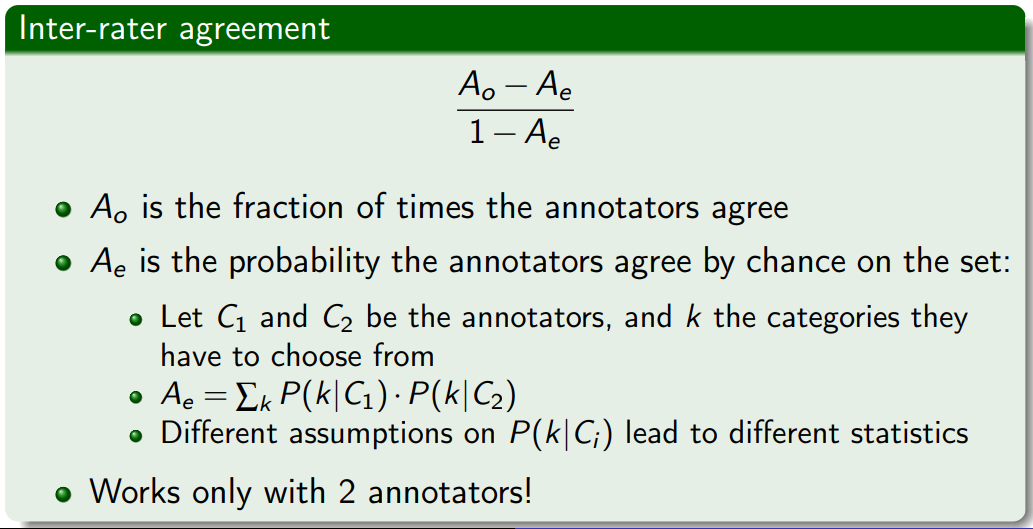
\includegraphics[width=0.5\linewidth]{internotersagreement.PNG}
    \caption{Formula per Agreement (A)}
    \label{fig:enter-label}
\end{figure}

Un modello è qualcosa che non esiste in natura costruito sulla realtà per fare delle predizioni; è un costrutto con cui noi esseri umani rappresentiamo il linguaggio, ad esempio un albero sintattico. Ma come ne giudichiamo la 'bontà'?

Consideriamo due o più persone (annotators) che si occupano di uno specifico task (linguistic) per testare il modello indipendentemente, se sono in accordo, allora questo potrebbe significare che il modello è simile alla rappresentazione del linguaggio che le persone hanno in mente. Come misuriamo il grado di agreement?

\end{abstract}

\section{Misurare la qualità di un sistema}
\begin{abstract}
Dati due sistemi S1 ed S2, vogliamo valutare la somiglianza fra i due, se sono effettivamente lo stesso sistema o meno.
I sistemi ricevono un determinato input C e formulano un risultato, un output simile implica che i due sistemi siano simili? Affichè le differenze rilevate siano statisticamente rilevanti, dobbiamo introdurre dei test significativi: \textbf{hypothesis tests}.

Ipotesi Nulla: H0:= le due distribuzioni sono uguali.
Ipotesi alternativa: Ha:= le due distribuzioni sono diverse.

Determinata l'ipotesi nulla cerchiamo di confutarla, impostando una soglia minima di verità (:= intervallo di confidenza).
Le procedure che si occupano di restituire la probabilità con cui l'ipotesi nulla viene rifiutata sono significance tests, di seguito riportiamo gli esempi di test presentati a lezione, tutti applicati al caso .

    \subsection{Sign Test}
    Supponiamo i due sistemi siano modelli di machine learning che vengono valutati sulla metrica di accuracy, su un determinato test set, o meglio, raccogliamo le accuracy dei sistemi per k volte, su batches differenti. (vabbe avete capito, tipo k-fold)
    S1: + + + + - - + - + -
    S2: - - - - + + - + - +
    E conservo il segno della differenza fra le due accuracy. Anche in questo caso affinchè i valori siano statistiche significativi è preferibile applicare tecniche stile bagging andando a simulare più batches.
    \subsection{Wilcoxon Test}
    Non l'ho capito molto bene e non so neanche se è stato fatto quest'anno, non credo.
    \subsection{Yeh (2000)}
    Considero un terzo sistema O, oracolo. anche qua non ho molti appunti.

\end{abstract}


\chapter{Parsing Sintattico}

\section{Per non dimenticare}
    \subsubsection{Context Free}
    Una grammatica libera dal contesto (o non contestuale, context-free o CFG) è una grammatica formale in cui ogni regola sintattica è espressa sotto forma di derivazione di un simbolo a sinistra a partire da uno o più simboli a destra.
    La grammatica formale, nella teoria dei linguaggi formali, è una struttura astratta che descrive un linguaggio formale in modo preciso, è cioè un sistema di regole che delineano matematicamente un insieme (di solito infinito) di sequenze finite di simboli (stringhe) appartenenti ad un alfabeto anch'esso finito.
    \subsubsection{Chomsky Normal Form}
    In formal language theory, a context-free grammar, G, is said to be in Chomsky normal form (first described by Noam Chomsky) if all of its production rules are of the form:
    
        A → BC,   or
        A → a,   or
        S → ε,
    
    where A, B, and C are nonterminal symbols, the letter a is a terminal symbol (a symbol that represents a constant value), S is the start symbol, and ε denotes the empty string. Also, neither B nor C may be the start symbol, and the third production rule can only appear if ε is in L(G), the language produced by the context-free grammar G.
    
    Every grammar in Chomsky normal form is context-free, and conversely, every context-free grammar can be transformed into an equivalent one which is in Chomsky normal form and has a size no larger than the square of the original grammar's size.

\section{CYK: Cocke-Younger-Kasami}
\begin{abstract}
Algoritmo di parsing per grammatiche \textbf{context free}, che utilizza il bottom-up parsing e la programmazione dinamica.
\end{abstract}

\section{Esempio su stringa visto a lezione 31/10/23}

    stringa: "baaba"

    \susubbsection{Regole Grammatica}
        \begin{itemize}
            \item{S -> AB}
            \item{S -> BC}
            \item{A -> BC}
            \item{A -> a}
            \item{B -> BB}
            \item{B -> CC}
            \item{B -> b}
            \item{C -> a}
        \end{itemize}

    \subsubsection{pseudo algoritmo}
    Lungo la diagonale principale inseriamo i simboli che possono generare i terminali sottostanti, (i,i) := terminale[i];
    
    (i,i+1) := combinazioni possibili di (i,i)x(i+1,i+1);
    (i,i+2) := (i,i)x(i+1,i+2) and (i,i+1)x(i+2,i+1);

    
    \begin{figure}
        \centering
        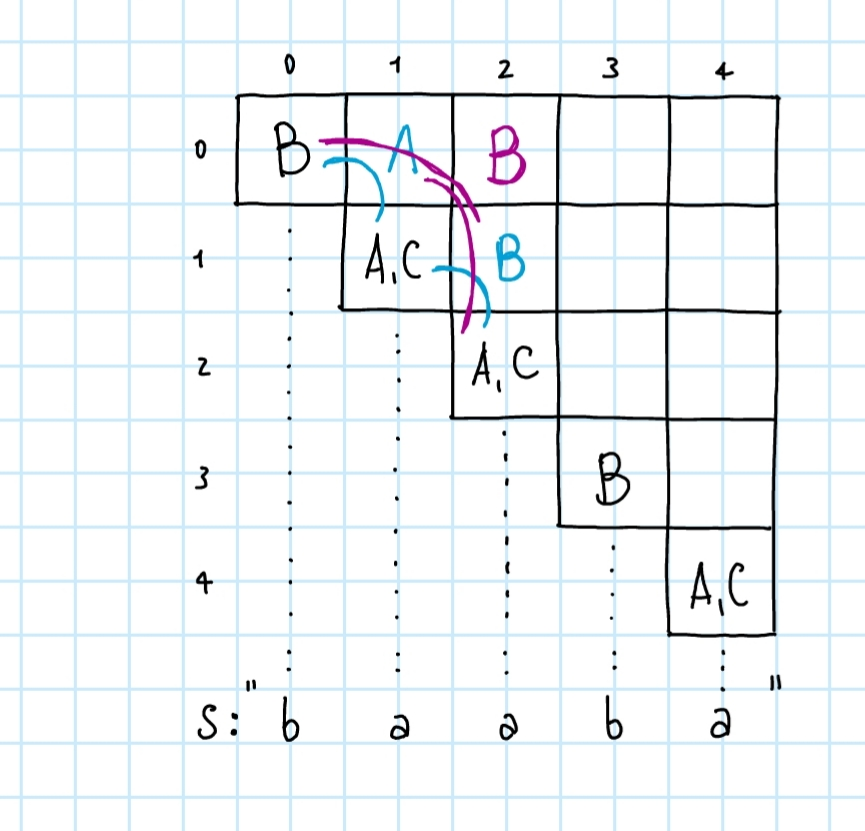
\includegraphics[width=0.5\linewidth]{20231130_165150.jpg}
        \caption{esempio visto a lezione sulla stringa "baaba"}
        \label{fig:enter-label}
        \centering
        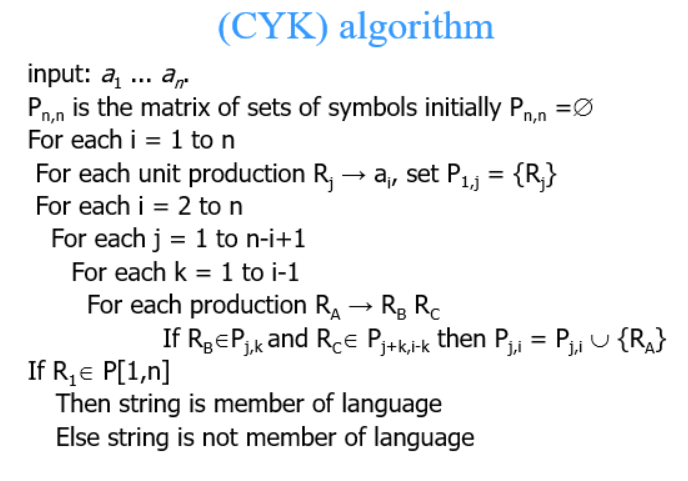
\includegraphics[width=0.5\linewidth]{cyk.PNG}
        \caption{codice algoritmo dalle slides}
        \label{fig:enter-label}
    \end{figure}
    

\section{Classificazione del linguaggio naturale secondo le gerarchie di Chomsky}
\begin{abstract}
L'analisi logica per come la conosciamo non è semplice, non dipende da posizioni (aggettivi prima e dopo il nome) o regole troppo inflessibili... ma anche la stessa tokenizzazione delle 'parole' può presentare problemi ( perchè dividere per spazi? il cinese non divide le parole con spazi ). Invece di cercare una relazione parentetica, guardiamo alle relazioni fra le parole. -> costruzione delle dipendenze
Come definiamo una \textbf{word}?

\begin{Oss}{Esempio:} Il lonfo non vaterca... \end{Oss}
\end{abstract}



%%%%%								APPENDICI
\newgeometry{top=35mm, bottom=35mm, left=15mm, right=15mm, headheight=0pt, headsep=0pt, marginparsep=0pt, marginparwidth=0pt, footskip=0pt, footnotesep=0pt}
\part*{\HUGE Appendici}
\titleformat{\chapter}[display]    	{\bfseries\large\raggedright}    	{\vspace{-2.35cm} \MakeUppercase{\chaptertitlename}\ \Huge \thechapter}    	{.125ex}    	{\raggedleft\vspace{-1cm}\Huge\makebox[.5\textwidth]{}}
\titlespacing*{\chapter}{0pt}{6\baselineskip}{2.5\baselineskip}
\restoregeometry

\pagestyle{fancyapp}

\begin{appendices}
	\chapter{}\label{AppendiceA}
	\blindduck[maths]


%%%%%%%%%%%%%%%%%%%%%%%%%%%%									BACKMATTER
%%%%%%%%%%%%%%%%%%%%%%%%%%%%
\backmatter

%%%%% 							BIBLIOGRAFIA
\pagestyle{fancyBibliografia}
\titleformat{\chapter}
	[hang]
	{\vspace{-2cm}\Huge}
	{}
	{0em}
	{}
	[\Large {\begin{tikzpicture} [remember picture, overlay]
	\pgftext[right,x=14.75cm,y=0.2cm]{\HUGE\bfseries 
	Bibliografia}
	\end{tikzpicture}}]
	
	\nocite{*}
	\bibliographystyle{amsalpha}
	\bibliography{FileAusiliari/Bibliografia}
	\addcontentsline{toc}{part}{Bibliografia}
\cleardoublepage

%INDICE ANALITICO
 \pagestyle{fancyIndiceAnalitico}
 	\renewcommand{\indexname}{}
	% SISTEMA IL PROBLEMA DEL LINK ALL'INDICE ANALITICO
	\let\cleardoublepage\relax
	\titleformat{\chapter}[hang]{}{}{0em}{}[]
 	\chapter*{}
	\titleformat{\chapter}
		[hang]
		{\Huge}
		{}
		{0em}
		{}
		[\Large {\begin{tikzpicture} [remember picture, overlay]
		\pgftext[right,x=14.75cm,y=0.2cm]{\HUGE\bfseries 
			Indice analitico}
		\end{tikzpicture}}]
	\titlespacing*{\chapter}{0pt}{0\baselineskip}{5\baselineskip}
	\addcontentsline{toc}{part}{Indice analitico}	
	\vspace{-2cm}
	\printindex
%%%%%%%%%%%%%%%%%%%%%%%%%%%%%%%%%%%%%%%%%%%%%%%%%%%%%%%%%%%%%%%%%%%%%%%%%%%%%%%%%%%%%%%%%%%%%%%%%%%%%%%%%%%%%%%%%
\end{appendices}
\end{document}